\documentclass[aspectratio=169,12pt]{beamer}
\usepackage[T1]{fontenc}
\usepackage{lmodern,booktabs,tikz}
\usetikzlibrary{arrows.meta,positioning}
\definecolor{Ink}{HTML}{17324D}
\definecolor{Teal}{HTML}{007F7B}
\definecolor{Gray}{HTML}{697887}
\definecolor{Soft}{HTML}{EEF3F6}
\definecolor{Warm}{HTML}{B55C32}
\setbeamercolor{normal text}{fg=Ink,bg=white}
\setbeamercolor{frametitle}{fg=Ink}
\setbeamercolor{structure}{fg=Teal}
\setbeamercolor{block title}{fg=white,bg=Teal}
\setbeamercolor{block body}{fg=Ink,bg=Soft}
\setbeamertemplate{navigation symbols}{}
\setbeamersize{text margin left=9mm,text margin right=9mm}
\setbeamerfont{frametitle}{size=\Large,series=\bfseries}
\setbeamertemplate{footline}{\hspace{9mm}\scriptsize Preliminary | Meeting: 30 Sep 2026 | Evidence: 29 Sep, 05:30 UTC\hfill\insertframenumber/\inserttotalframenumber\hspace{9mm}\vspace{3mm}}
\newcommand{\aside}[1]{\vfill{\footnotesize\color{Gray}#1\par}}
\hypersetup{pdftitle={Teaching models to choose useful steps},pdfauthor={Alex Towell}}
\begin{document}

\begin{frame}[t]
\frametitle{Can a model learn useful steps for an unfamiliar task?}
A recursive language model (RLM) can use code and ask another model to handle a smaller task. A helper can, in turn, ask its own helper.
\vspace{4mm}
\begin{center}
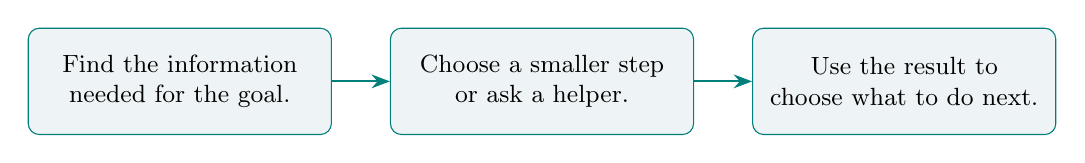
\begin{tikzpicture}[>=Stealth,font=\small,
 box/.style={draw=Teal,rounded corners,fill=Soft,text width=3.45cm,align=center,minimum height=1.35cm,inner sep=2mm}]
\node[box] (learn) at (0,0) {Find the information\\needed for the goal.};
\node[box] (choose) at (4.6,0) {Choose a smaller step\\or ask a helper.};
\node[box] (check) at (9.2,0) {Use the result to\\choose what to do next.};
\draw[->,thick,Teal] (learn)--(choose);
\draw[->,thick,Teal] (choose)--(check);
\end{tikzpicture}
\end{center}
\medskip
Our immediate question is simpler: \textbf{can we teach a small model to choose a useful next action from what it has actually seen?}
\aside{The strongest result so far concerns learning from examples. We have not yet shown that recursive helpers improve the whole task.}
\end{frame}

\begin{frame}[t]
\frametitle{A crafting game makes the outcome easy to check.}
In TextCraft, the model looks up recipes and makes items. The game checks whether the requested items really exist in its inventory.
\vspace{3mm}
\begin{columns}[T,onlytextwidth]
\begin{column}{.48\textwidth}
\textbf{Goal: make one lantern.}
\begin{center}
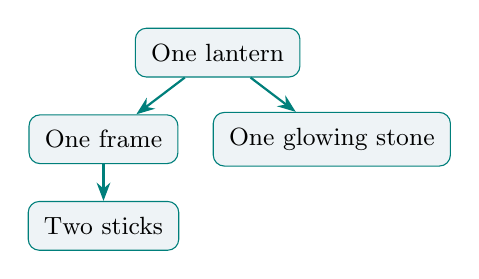
\begin{tikzpicture}[>=Stealth,font=\small,
 item/.style={draw=Teal,rounded corners,fill=Soft,align=center,inner sep=2mm}]
\node[item] (lamp) at (0,0) {One lantern};
\node[item] (frame) at (-1.45,-1.1) {One frame};
\node[item] (stone) at (1.45,-1.1) {One glowing stone};
\node[item] (sticks) at (-1.45,-2.2) {Two sticks};
\draw[->,Teal,thick] (lamp)--(frame);
\draw[->,Teal,thick] (lamp)--(stone);
\draw[->,Teal,thick] (frame)--(sticks);
\end{tikzpicture}
\end{center}
{\small Arrows mean ``needs.''}
\end{column}
\begin{column}{.47\textwidth}
\textbf{Start with two sticks and one glowing stone.}
\medskip

1. Look up the lantern and frame recipes.
\medskip

2. Make the frame from the sticks.
\medskip

3. Combine the frame and stone into a lantern.
\end{column}
\end{columns}
\aside{Simplified illustration, not a recorded task. Real tests use unfamiliar item names and longer chains.}
\end{frame}

\begin{frame}[t]
\frametitle{We test two ways of teaching the model.}
Both change the model through training. The difference is the feedback it receives.
\vspace{4mm}
\begin{columns}[T,onlytextwidth]
\begin{column}{.48\textwidth}
\begin{block}{Worked examples (SFT)}
We show a goal, observations, and a correct next action.
\medskip

\textit{``The lantern needs a frame. Look up the frame recipe.''}
\medskip

The model learns to choose that action.
\end{block}
\end{column}
\begin{column}{.48\textwidth}
\begin{block}{Task rewards (RL)}
The model tries the task. The game checks success.
\medskip

\textit{``Did it actually make the lantern?''}
\medskip

Training favors attempts with better rewards.
\end{block}
\end{column}
\end{columns}
\aside{SFT means supervised fine-tuning; RL means reinforcement learning. Our reward-training runs start from a model already trained on worked examples.}
\end{frame}

\begin{frame}[t]
\frametitle{We changed the information shown before the action.}
We reordered existing recipe lookups, then rebuilt what the learner sees before each action.
\vspace{2mm}
\begin{center}
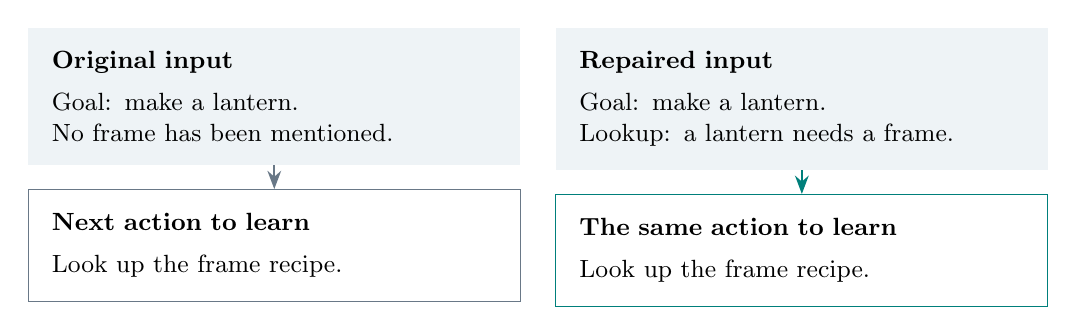
\begin{tikzpicture}[font=\small,>=Stealth]
\node[anchor=north west,align=left,text width=5.65cm,fill=Soft,inner sep=3mm] (before) at (0,0) {\textbf{Original input}\par\vspace{1.5mm}Goal: make a lantern.\\No frame has been mentioned.};
\node[anchor=north west,align=left,text width=5.65cm,fill=Soft,inner sep=3mm] (after) at (6.7,0) {\textbf{Repaired input}\par\vspace{1.5mm}Goal: make a lantern.\\Lookup: a lantern needs a frame.};
\node[anchor=north west,align=left,text width=5.65cm,draw=Gray,inner sep=3mm] (a) at ([yshift=-3mm]before.south west) {\textbf{Next action to learn}\par\vspace{1.5mm}Look up the frame recipe.};
\node[anchor=north west,align=left,text width=5.65cm,draw=Teal,inner sep=3mm] (b) at ([yshift=-3mm]after.south west) {\textbf{The same action to learn}\par\vspace{1.5mm}Look up the frame recipe.};
\draw[->,thick,Gray] (before.south)--(a.north);
\draw[->,thick,Teal] (after.south)--(b.north);
\end{tikzpicture}
\end{center}
We keep the same demonstrated actions and the same number of training updates.
\aside{Illustration. The repair uses an existing solution. Input histories and their lengths change; computing work is not held exactly equal.}
\end{frame}

\begin{frame}[t]
\frametitle{The repair helped after retraining and on more goals.}
Successful attempts out of 32, with the same demonstrated actions and number of training updates:
\vspace{1mm}
\begin{center}
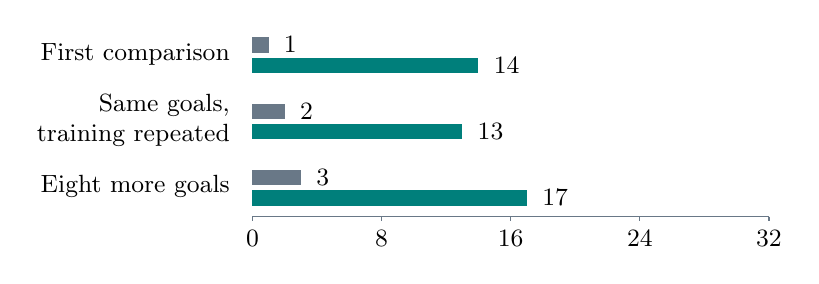
\begin{tikzpicture}[x=.205cm,y=.35cm,font=\small]
\node[anchor=east,align=right] at (-.8,5.35) {First comparison};
\node[anchor=east,align=right] at (-.8,2.95) {Same goals,\\training repeated};
\node[anchor=east,align=right] at (-.8,.55) {Eight more goals};
\fill[Gray] (0,5.4) rectangle (1,5.95);
\fill[Teal] (0,4.65) rectangle (14,5.2);
\fill[Gray] (0,3) rectangle (2,3.55);
\fill[Teal] (0,2.25) rectangle (13,2.8);
\fill[Gray] (0,.6) rectangle (3,1.15);
\fill[Teal] (0,-.15) rectangle (17,.4);
\node[anchor=west] at (1.35,5.68) {1};
\node[anchor=west] at (14.35,4.93) {14};
\node[anchor=west] at (2.35,3.28) {2};
\node[anchor=west] at (13.35,2.53) {13};
\node[anchor=west] at (3.35,.88) {3};
\node[anchor=west] at (17.35,.13) {17};
\draw[Gray] (0,-.55)--(32,-.55);
\foreach \n in {0,8,16,24,32} {\draw[Gray] (\n,-.55)--(\n,-.7);\node[below] at (\n,-.7) {\n};}
\end{tikzpicture}
\end{center}
{\small\color{Gray}\rule{4mm}{2mm} Original examples\qquad\color{Teal}\rule{4mm}{2mm} Repaired examples}
\medskip

{\small There are \textbf{16 distinct goals across this chart}, with repeated attempts and changed recipes. The first two rows reuse the same goals.}
\aside{These are small exploratory comparisons with Qwen3-4B. More training also helps the original examples. The result is better learning at the tested budgets, not a universal advantage.}
\end{frame}

\begin{frame}[t]
\frametitle{Reward training showed little transfer so far.}
Successes before $\to$ after one reward-based training update, out of 16 attempts:
\vspace{3mm}
\begin{center}
\renewcommand{\arraystretch}{1.3}
\begin{tabular}{lcc}
\toprule
Tool setting & Familiar goals & Different goals\\
\midrule
Model writes ingredient list & $9 \to 13$ & $4 \to 5$\\
Code fills ingredient list & $14 \to 16$ & $5 \to 5$\\
\bottomrule
\end{tabular}
\end{center}
Familiar goals were used in this reward-training update. The other target items were excluded, but component recipes may overlap.
\medskip

Each column has eight goals and two attempts per goal. Compare the before-and-after change \textbf{within} a column; their difficulty differs.
\aside{Code uses recipes already observed; the model still chooses what and how much to make. This is one update per setting, not evidence that RL cannot generalize. More varied training and extra SFT are being tested.}
\end{frame}

\begin{frame}[t]
\frametitle{Does a helper improve the whole task?}
RLMs already support helpers. Here we test whether one helper earns its cost.
\vspace{3mm}
\begin{columns}[T,onlytextwidth]
\begin{column}{.46\textwidth}
\begin{block}{Work alone.}
The main model looks up recipes, makes the frame, and assembles the lantern.
\end{block}
\end{column}
\begin{column}{.50\textwidth}
\begin{block}{Use one helper.}
A programmed rule assigns a helper: ``Make one frame.''
\smallskip

The helper reports success or what prevented completion.
\smallskip

The main model resumes with the updated inventory.
\end{block}
\end{column}
\end{columns}
\medskip
The original goal must succeed, not just the helper's subtask.
\aside{Planned test, not a result. Both share the same total allowance for model calls and generated text. The first rules for using a helper are programmed, not learned.}
\end{frame}

\begin{frame}[t]
\frametitle{The strongest lead is better worked examples.}
\begin{block}{A possible focused paper}
Repair what a learner sees before each demonstrated action, while keeping the taught actions fixed. Test when that makes learning more effective.
\end{block}
\medskip
\textbf{Next evidence we need:} test the repair in another model family and on fresh goals and recipes. Compare broader reward training with more worked examples.
\medskip

\textbf{The RLM question remains:} does delegating a useful part improve the whole task before we add deeper recursion?
\medskip

\textbf{For discussion:} Would broader transfer or a clearer explanation of the teaching effect make the stronger first paper?
\aside{Prior work already studies what teachers and learners know. The candidate contribution is this controlled repair and its evidence, not the general idea. All results remain preliminary.}
\end{frame}
\end{document}
